

%%%%%%%%%%%%
%
% $Autor: Wings $
% $Datum: 2019-03-05 08:03:15Z $
% $Pfad: ParallelPort.tex $
% $Version: 4250 $
% !TeX spellcheck = en_GB/de_DE
% !TeX encoding = utf8
% !TeX root = filename 
% !TeX TXS-program:bibliography = txs:///biber
%
%%%%%%%%%%%%

\chapter{ParallelPort}

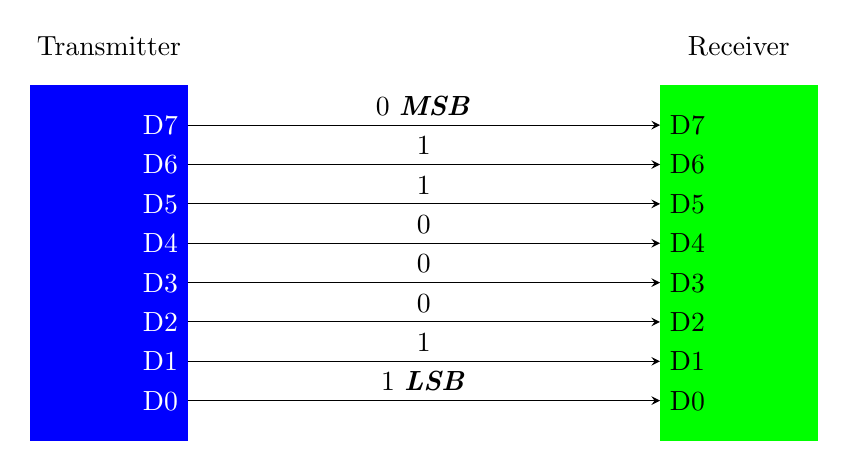
\begin{tikzpicture}

  % Left Rectangle (Blue)
  \draw[blue, fill=blue] (0,0) rectangle (2,4.5);
    \node[black] at (1,5) {Transmitter};

  % Right Rectangle (Green)
  \draw[green, fill=green] (8,0) rectangle (10,4.5);
  \node[black] at (9,5) {Receiver};

  % Connecting Line D0
  \draw[->, >=stealth, fill=black] (2,0.5) node[left] {\textcolor{white}{D0}} --  node[above, midway] {1 \textbf{\textit{LSB}}} (8,0.5) node[right] {D0} ;
  
    % Connecting Line D1
  \draw[->, >=stealth, fill=black] (2,1) node[left] {\textcolor{white}{D1}} --  node[above, midway] {1} (8,1) node[right] {D1} ;

    % Connecting Line D2
  \draw[->, >=stealth, fill=black] (2,1.5) node[left] {\textcolor{white}{D2}} --  node[above, midway] {0} (8,1.5) node[right] {D2} ;
  
      % Connecting Line D3
  \draw[->, >=stealth, fill=black] (2,2) node[left] {\textcolor{white}{D3}} --  node[above, midway] {0} (8,2) node[right] {D3} ;
  
      % Connecting Line D4
  \draw[->, >=stealth, fill=black] (2,2.5) node[left] {\textcolor{white}{D4}} --  node[above, midway] {0} (8,2.5) node[right] {D4} ;
  
      % Connecting Line D5
  \draw[->, >=stealth, fill=black] (2,3) node[left] {\textcolor{white}{D5}} --  node[above, midway] {1} (8,3) node[right] {D5} ;
  
      % Connecting Line D6
  \draw[->, >=stealth, fill=black] (2,3.5) node[left] {\textcolor{white}{D6}} --  node[above, midway] {1} (8,3.5) node[right] {D6} ;
  
      % Connecting Line D7
  \draw[->, >=stealth, fill=black] (2,4) node[left] {\textcolor{white}{D7}} --  node[above, midway] {0 \textbf{\textit{MSB}}} (8,4) node[right] {D7} ;
  
\end{tikzpicture}



